\chapter{Detecting Isolation Bugs in DBMSs via Dependency Graphs Construction}

\section{Introduction and Motivation}

As discussed in the previous chapter, and in various other works \cite{jiang2023detecting,cui2024understanding_ICSE2024,dou2023detecting_ICSE2023,clark2024validating,cui2022differentially_ASE2022}, isolation bugs are a prevalent problem in DBMSs, due to the inherent tradeoff between performance (under the form of concurrency) and isolation.

Modern database systems usually express isolation guarantees under a \textit{locking behaviour}, which is a set of rules dictating how tables and rows are locked during transactions. However, due to the sheer complexity of modern DBMSs, ensuring a correct locking behaviour is challenging, due to a combination of factors such as:

\begin{itemize}
    \item DBMS systems are complex, with multiple components interacting with each other, such as the query planner, the storage engine, the transaction manager, etc. A bug in any of these components can lead to an isolation bug.
    \item The performance of DBMSs is subject to the law of diminishing returns, requiering more and more complex optimizations to achieve smaller and smaller performance gains. This makes it more likely for bugs to be introduced.
    \item Higher concurrency leads to better performance, thus making a reduction in the number of locks desirable. However, this also makes it more likely for isolation bugs to occur.
\end{itemize}

As \textit{isolation bugs} are not neccessarily \textit{logic bugs}, i.e. not bugs in the traditional sense but rather a violation of the isolation guarantees, hunting them with standard bug-finding techniques is challenging:

\begin{itemize}
    \item Testing high concurrency workloads, required for capturing edge cases where isolation bugs occur, is hard to achieve due to an exponential growth in the number of possible states.
    \item DBMSs are not fully compatible with each others, and concurrent workloads are inherintly non-deterministic, making it hard to check for bugs by exploring differences between DBMSs.
    \item Semi-automatic techniques such as \textit{Fuzzing} require an \textit{oracle} to determine if the output is correct, which is hard to achieve in the case of isolation bugs.
\end{itemize}

Current techniques avoid these problems by using a white-box testing approach \cite{clark2024validating}, using the database system itself as a testing oracle \cite{jiang2023detecting}, or running workloads on multiple DBMSs to check for disparities \cite{cui2022differentially_ASE2022}.

In this chapter, we introduce a novel bug-finding technique, which leverages Direct Serialization Graphs (DSG) introduced by Adya, A. \cite{adya1999weak} and SQL-level instrumentation introduced by Jiang, Z. \cite{jiang2023detecting}. This technique is a modification of the one used by Jiang, Z.. We also implement a tool based on our technique on top of \textit{TxCheck}, which we modify to suit our needs.


\section{Database Model Used}

For testing the correct behaviour of database systems, we need well-defined specifications we can test against. While some techniques rely on the DBMSs themselves for self-validating or cross validating results \cite{cui2022differentially_ASE2022}, other bug-finding techniques express DBMS isolation bugs as violated constraints in the Direct Serialization Graph (DSG) built following  Adya's data model \cite{jiang2023detecting,clark2024validating}, directed labeled graphs in which nodes are tranzactions and directed edges are dependencies.

In particular, \textit{TxCheck}, which this project builds on, uses a mixture of both methods:
\begin{itemize}
    \item Using \textit{SQL instrumentation}, \textit{TxCheck} extracts a supergraph of the DSG. However, the dependency checking technique used is not perfect, and can create sporadic dependencies.
    \item Using the DSG, \textit{TxCheck} creates and executes an equivalent execution trace using a single transaction on the same DBMS, which is used as an oracle for comparing the results.
\end{itemize}

In this work, we rely on the Direct Serialization Graph (DSG) data model introduced by Adya, A. \cite{adya1999weak}, and on the SQL-level instrumentation technique introduced by Jiang, Z. \cite{jiang2023detecting}.

\section{Contributions}

Our two main contributions are:

\begin{itemize}
    \item We build on the theory behind the DSG extraction used in \textit{TxCheck}, for allowing for a complete and sound extraction of all the DSG dependencies, by leveraging the \textit{SQL instrumentation} technique \textit{TxCheck} introduced. Our approach allows for an accurate extraction of the DSG edges, which avoids the sporadic dependencies created by the original technique, and allows for a more accurate detection of isolation bugs.
    \item We implement the changes in the \textit{TxCheck} project, giving \textit{TxCheck} the ability to extract the DSG edges accurately.
\end{itemize}


\section{Background on DSG Dependencies}

Throughout this work, we heavily reuse the definitions and notations introduced by Adya, A. \cite{adya1999weak}. The most important definitions are the ones regarding the dependencies between transactions, which we outline below.

\begin{definition}
    \label{def:overwriting}
    \textbf{Overwriting a Predicate}: $T_j$ overwrites an operation $r_i(P: Vset(P))$ or $w_i(P: Vset(P))$ if:
    \begin{itemize}
        \item $T_j$ installs a version $x_j$ for some object $x$.
        \item The version $x_k$ of $x$ present in $Vset(P)$ is an earlier version than $x_j$.
        \item $x_j$ matches the predicate $P$ and $x_k$ does not, or vice versa.
    \end{itemize}  
\end{definition}

\begin{definition}
    \textbf{Directly Item-Read-Depends}: $T_j$ \textit{directly item-read-depends} on $T_i$ if $T_j$ reads an some object version instaleld by $T_i$.
\end{definition}

\begin{definition}
    \textbf{Directly Predicate-Read-Depends}: $T_j$ \textit{directly predicate-read-depends} on $T_i$ if $T_j$ performs a read operation $r_j(P: Vset(P))$ and $T_i$ installs $x_i$ such that $x_i \in Vset(P)$.
\end{definition}

\begin{definition}
    \textbf{Directly Read-Depends}: $T_i$ \textit{directly read-depends} on $T_j$ if $T_i$ directly item-read-depends or directly predicate-read-depends on $T_j$.
\end{definition}

\begin{definition}
    \textbf{Directly Item-Anti-Depends}: $T_j$ \textit{directly item-anty-depends} on $T_i$ if $T_i$ reads some object version $x_k$ and $T_j$ installs a later version $x_j$.
\end{definition}

\begin{definition}
    \textbf{Directly Predicate-Anti-Depends}: $T_j$ \textit{directly predicate-anti-depends} on $T_i$ if $T_j$ overwrites the predicate of an operation $r_i(P: Vset(P))$. %  or $w_i(P: Vset(P))$.
\end{definition}

\begin{definition}
    \textbf{Directly Anti-Depends}: $T_i$ \textit{directly anti-depends} on $T_j$ if $T_i$ directly item-anti-depends or directly predicate-anti-depends on $T_j$.
\end{definition}

\begin{definition}
    \textbf{Directly Item-Write-Depends}: $T_j$ \textit{directly item-write-depends} on $T_i$ if $T_i$ installs a version $x_i$ and $T_j$ installs the next version $x_j$.
\end{definition}

\begin{definition}
    \textbf{Directly Predicate-Write-Depends}: $T_j$ \textit{directly predicate-write-depends} on $T_i$ if:
    \begin{itemize}
        \item $T_j$ overwrites an operation $w_i(P: Vset(P))$, or
        \item $T_j$ executes an operation $w_j(P: Vset(P))$ and $T_i$ installs some version $x_i \in Vset(P)$.
    \end{itemize}
\end{definition}

\begin{definition}
    \textbf{Directly Write-Depends}: $T_i$ \textit{directly write-depends} on $T_j$ if $T_i$ directly item-write-depends or directly predicate-write-depends on $T_j$.
\end{definition}

The steps for building the DSGs given an ordered sequence of statements (each belonging to a possibly different transaction) are as follows:
\begin{enumerate}
    \item Run the statements sequencialy, saving the versions of the objects at each step.
    \item Extract the \textit{Direct Read Dependencies}, \textit{Direct Write Dependencies} and \textit{Direct Anti-Dependencies} between transactions.
    \item Build the DSGs using the extracted dependencies.
\end{enumerate}

The second step is the hardest, due to the inherent lack of information a DBMS provides about the internal state of the system. This is where SQL-level instrumentation comes in.

\section{SQL-level Instrumentation}

\subsection{Intuition Behind SQL-level Instrumentation}

The most straight-forward way to extract DSG dependencies is to modify the source code of DBMSs, exposing the internal state of the system. This allows for a relatively simple extraction of dependencies, as the injected code has access to all of the instruction scheduling, existing locks, state of the key-value store, etc. This is how Clark, J. et al. extract the DSGs in their work \cite{clark2024validating}.

A less intrusive approach, which considers the DBMS as a black box (thus being easily ported across different systems), is to use SQL-level instrumentation, a technique pioneered by Jiang, Z., which consists of sistematically exposing the internal state of the DBMS by injecting \textit{SELECT} statements in the SQL queries \cite{jiang2023detecting}.

The informal intuition behind SQL-level instrumentation is that we want to know the current state of the database, but lack the white-box access to the DBMS internals. As we can only query the database, we infer the dependencies by injecting \textit{SELECT} statements in testcases. We instrument the SQL queries by adding instrumentation code right before and right after each original SQL statement.

A few challenging parts are:

\begin{itemize}
    \item Ensuring the instrumentation code is not interupted by locking or other operations. This is addressed by re-ordering statements in the testcase, and erasing them if no viable scheduling order can be found.
    \item Ensuring that every table of the database stores a \textit{version} column, which stores the version of the object, required for understanding the view a statement has access to. This is addressed by adding a \textit{version} column to each table.
    \item Concurrency issues, such as the non-deterministic locking and unlocking behaviour of transactions. This is addressed by spacing out the statements, and ensuring that no transaction locking takes place.
\end{itemize}


\subsection{Intrumentation Statements}

We intrument SQL statements by encapsulating them with instrumentation placed before and after statements, which expose the tranzaction's view of the database. As we built on top of \textit{TxCehck}, the instrumentation we use is very similar to the original one, with the addition of $3$ new instrumentation types. The instrumentation types we use are:

\begin{itemize}
    \item \textbf{Before Write Read (BWR)}: Before a write operation, a \textit{SELECT} statement is added to read the version of overwritten objects.
    \item \textbf{After Write Read (AWR)}: After a write operation, a \textit{SELECT} statement is added to read the new version of the overwritten objects.
    \item \textbf{Version Set Read (VSR)}: Before reads and predicated statements, a \textit{SELECT} statement is added to read the version set of all objects in the used tables.
    \item \textbf{Before Predicate Match (BPM)}: Before a write operation, a \textit{SELECT} statement is added for each predicate that appears in the testcase, to read the objects and versions that match the predicate.
    \item \textbf{After Predicate Match (APM)}: Similar to the \textit{Before Predicate Match}, but is inserted after the write operation.
    \item \textbf{Predicate Match (PM)}: Before an operation that contains a predicate, a \textit{SELECT} statement reading the objects and versions that match the predicate is added.
\end{itemize}

This instrumentation has the potential of instroducing unwanted locking behaviour (i.e. the \textit{SELECT} statements cause table locks), which is why we need to ensure that the instrumentation code is not interrupted by locking or other operations. In Figure \ref{fig:sql_instrumentation_sample}, we show the instrumentation of a trivial testcase.

\begin{figure}[!h]
    \centering
    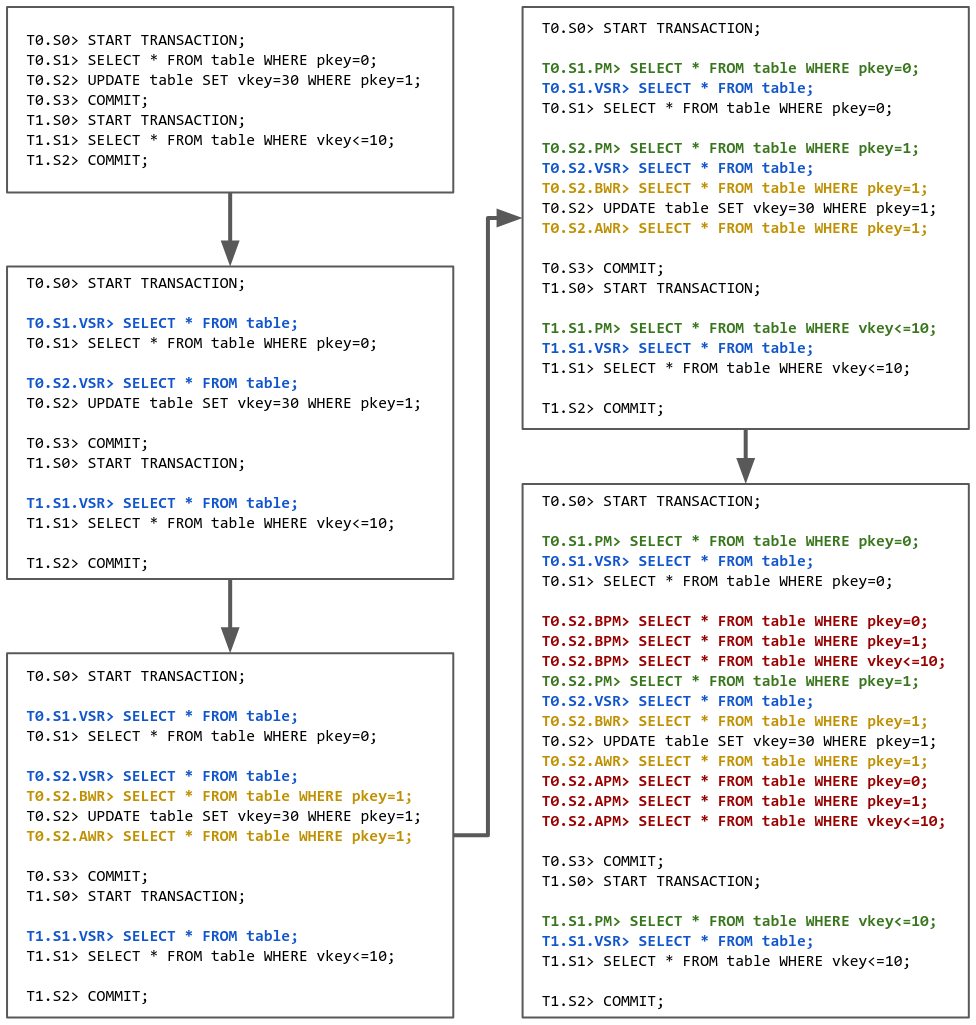
\includegraphics[width=\linewidth]{assets/sql_instrumentation_sample.png}
    \caption{Instrumentation of a (simplified) testcase.}
    \label{fig:sql_instrumentation_sample}
\end{figure}



\section{Extracting the DSG with SQL Instrumentation}

\subsection{Methodology}

Our tool is based on \textit{TxCheck} \cite{jiang2023detecting}, which we modify to suit our needs. Our dependency extraction process is thus similar to the one used in \textit{TxCheck}, with slight modification, which are centered around anti-dependencies. As such, we will not go into detail about the direct read dependencies, direct item anti-dependencies, and direct item write dependencies, as they are similar to the ones used by Jiang, Z. \cite{jiang2023detecting}, where a complete and sound technique for extracting them is described, and will focus on the direct predicate anti dependencies and predicate write dependencies.

Given a testcase consisting of intertwined transactions, we do the following:

\begin{itemize}
    \item Add instrumentation statements to the SQL queries.
    \item Ensure that the instrumentation code is not interrupted by locking or other operations.
    \item Run the testcase, saving the results of the \textit{SELECT} statements.
    \item Extract the DSG edges with the help of the instrumentation results. 
\end{itemize}

The \textit{Predicate Match}, \textit{Before Predicate Match} and \textit{After Predicate Match} statements are used to extract the \textit{Overwrites}, which happen when a transaction overwrites the predicate of another transaction (see definition \ref{def:overwriting}).

\subsection{Extracting Overwrites}

For any two statements $A$ and $B$, where $A$ is a write operation and $B$ contains a predicate, we can check if $A$ \textit{overwrites} $B$ if there exist a primary $pk$ such that:
\begin{itemize}
    \item The \textit{After Write Read} instrumentation of $A$ contains a record with the primary key $pk$ and a version key $v$.
    \item The \textit{Version Set Read} instrumentation of $B$ contains a record with the primary key $pk$ and a version $v'$ such that $v'$ happens before $v$ in the list of versions for the primary key $pk$.
    \item The \textit{Before Predicate Match} instrumentation of $A$ for the predicate of $B$ and the \textit{Predicate Match} instrumentation of $B$ contain $pk$, but the \textit{After Predicate Match} instrumentation of $A$ for the predicate of $B$ does not, or the other way around.
\end{itemize}

Note that if $B$ contains multiple predicates, we need to check for each predicate if $A$ overwrites $B$.

\begin{proof}
We prove that our method for extracting overwrites is both sound and complete.

\textit{Soundness}: If we flag $A$ as \textit{overwriting} $B$, then there exists a primary $pk$ and two versions $v$ and $v'$ such that $v$ is the version of $pk$ installed by $A$, $v'$ is the version of $pk$ present in the version set of $B$, and $v$ happens after $v'$ in the list of versions for $pk$. Furthermore, the \textit{Before Predicate Match} instrumentation of $A$ for the predicate of $B$ contains $pk$, but the \textit{After Predicate Match} instrumentation of $A$ for the predicate of $B$ does not, or the other way around, meaning that $A$ makes $pk$ no longer match the predicate of $B$ or the other way around. This is the definition of an \textit{overwrite}.

\textit{Completeness}: If $A$ overwrites $B$, then there exists a record $x$ for which $A$ installs a version later than the one seen by $B$, and the two versions do not match the predicate of $B$. If we call the primary key of $x$ $pk$, the version installed by $A$ $v$, and the version seen by $B$ $v'$, then $v$ happens after $v'$ in the list of versions for $pk$, and the \textit{Before Predicate Match} instrumentation of $A$ for the predicate of $B$ contains $pk$, but the \textit{After Predicate Match} instrumentation of $A$ for the predicate of $B$ does not, or the other way around. This means that our technique correctly identifies $A$ as overwriting $B$.
\end{proof}

\subsection{Extracting Predicate Write Dependencies}

Being able to check if one statement overwrites another, we can trivially extract \textit{direct predicate anti-dependies} by checking if a write statement overwrites the predicate of a read statement.

\begin{proof}
    Let $A$ be a write statement and $B$ be a read statement. If $A$ overwrites $B$, then the transaction containing $A$ by definition \textit{directly predicate anti-depends} on the transaction containing $B$.
\end{proof}

\subsection{Extracting Direct Predicate Write Dependencies}

In a similar way, we can extract the \textit{direct predicate write dependencies} by checking that:
\begin{itemize}
    \item The \textit{After Write Read} of a transaction intersects with the \textit{Version Set Read} of a predicated write statement of another transaction, or
    \item One transaction overwrites the predicate of another write transaction.
\end{itemize}

\begin{proof}
    We prove that our method for extracting direct predicate write dependencies is both sound and complete.

    \textit{Soundness}: If we flag $A$ as \textit{directly predicate write-depending} on $B$, then:
    \begin{itemize}
        \item The \textit{After Write Read} of $A$ intersects with the \textit{Version Set Read} of $B$, and $B$ is a predicated write. This means that $A$ installs a version that is read by $B$, so $A$ \textit{directly predicate write-depends} on $B$, or
        \item $A$ overwrites the predicate of $B$, so $A$ \textit{directly predicate write-depends} on $B$.
    \end{itemize}

    \textit{Completeness}: If $A$ \textit{directly predicate write-depends} on $B$, then:
    \begin{itemize}
        \item $A$ installs a version that is read by $B$, which means that the \textit{After Write Read} of $A$ intersects with the \textit{Version Set Read} of $B$, so we flag $A$ as \textit{directly predicate write-depending} on $B$, or
        \item $A$ overwrites the predicate of $B$, so we flag $A$ as \textit{directly predicate write-depending} on $B$.
    \end{itemize}
\end{proof}

\section{Implementation and Results}

We implement our technique on top of \textit{TxCheck}, which we modify to suit our needs. As we are only looking for isolation bugs, we do not need to run the single-transaction \textit{TxCheck} uses as an oracle, so we bypass that part of the code.

The main changes we make to \textit{TxCheck} are:
\begin{itemize}
    \item Update the project to bring it to a working state: \textit{TxCheck} relies on \textit{Docker} images of \textit{Ubuntu 20.04}, on which some dependencies of the project are not available. We fix the broken dependencies, and make the project runnable.
    \item Add the new \textit{Before Predicate Match}, \textit{After Predicate Match} and \textit{Predicate Match} instrumentation types.
    \item Modify the dependency extraction code to create a complete and sound extraction of the DSG dependencies.
    \item Modify the bug minimization code to include support for the new instrumentation types.
    \item Add additional tests based on Adya's theory \cite{adya1999weak} for detecting isolation bugs, which were not previously possible due to the sporadic dependencies created by the original technique.
\end{itemize}

The fuzzing approach of our technique is similar to the one used by \textit{TxCheck}, with the main difference being the ability to extract the DSG dependencies accurately, thus making the \textit{graph decycling} phase of \textit{TxCheck}, used to remove circular dependencies assumed to be false positives, unnecessary. This means that, while our approach and \textit{TxCheck} share most of the implementation and work in a similar way, the two are quite different in the way they find bugs:
\begin{itemize}
    \item Our approach relies on properties of the DSG to find isolation bugs.
    \item \textit{TxCheck} checks a few properties of the DSG, but mainly relies on the single-transaction oracle to find bugs, as the DSG extraction used is not sound.
\end{itemize}

\section{Limitations and Future Work}

Our technique is a complete and sound method of extracting of the DSG dependencies, and a step forward in the direction of behaviour-based DBMS testing. However, it suffers from similar limitations as the original technique used by \textit{TxCheck}:
\begin{itemize}
    \item The fuzzing is quite slow, with the testcase generation and finding a non-blocking schedule being the bottleneck.
    \item While our technique is able to run under any of the isolation levels supported by the DBMS, the lower the isolation level the less checks we can perform, as the DSG has less restrictions. In particular, the \textit{Read Uncommitted} isolation level imposes almost no restrictions on the DSG, which makes it hard to find bugs.
\end{itemize}

We only implemented support \textit{SELECT}, \textit{UPDATE} and \textit{INSERT} statements. However, support for the \textit{DELETE} statements is also possible. The main caveat is that \textit{DELETE} removes entries from tables TODO

\section{Conclusion}

